\documentclass[tikz,border=5pt]{standalone}
\usetikzlibrary{calc}
\usepackage{amsmath}

\begin{document}
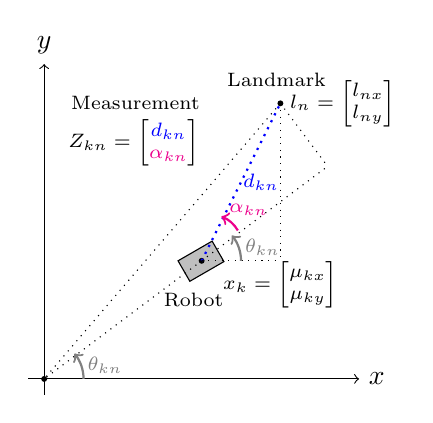
\begin{tikzpicture}[node distance=1.5cm, auto]

    % Axes
    \coordinate (origin) at (0,0);
    \draw[fill] (origin) circle (0.03);
    \draw[->] (-0.2,0) -- (4,0) node[right] {\( x \)};
    \draw[->] (0,-0.2) -- (0,4) node[above] {\( y \)};

    % Robot
    \coordinate (robot) at (2,1.5);
    \coordinate (offset) at ($(robot) + (-0.3,0)$);
    \draw[fill=lightgray, rotate around={30:(offset)}] (offset) rectangle ++(0.5,-0.3);
    \draw[fill] (robot) circle (0.03) node[below=0.3cm, right=0.15cm] {\scriptsize \( x_k = \begin{bmatrix} \mu_{kx} \\ \mu_{ky} \end{bmatrix} \)};
    \node[below=0.5cm, left=-0.4cm] at (robot) {\scriptsize Robot};

    % Landmark
    \coordinate (landmark) at (3,3.5);
    \draw[fill] (landmark) circle (0.03) node[right] {\scriptsize \( l_n = \begin{bmatrix} l_{nx} \\ l_{ny} \end{bmatrix} \)};
    \node[above=0.3cm, right=-0.8cm] at (landmark) {\scriptsize Landmark};

    % Lines
    \draw[dotted] (robot) -- (origin);
    \draw[dotted] (landmark) -- (origin);
    \draw[dotted, thick, blue] (robot) -- (landmark) node[midway, right=-3] {\scriptsize \( d_{kn} \)};
    \draw[dotted] (robot) -- (landmark |- robot);
    \draw[dotted] (landmark) -- (landmark |- robot);
    \draw[dotted] (robot) -- ($(origin)!(landmark)!(robot)$);
    \draw[dotted] (landmark) -- ($(origin)!(landmark)!(robot)$);

    % Angles
    \draw[->, gray, thick] (origin) ++(0:0.5) arc (0:40:0.5) node[midway, right=-0.05cm] {\scriptsize \( \theta_{kn} \)};
    \draw[->, gray, thick] (robot) ++(0:0.5) arc (0:40:0.5) node[midway, right=-0.05cm] {\scriptsize \( \theta_{kn} \)};
    \draw[->, magenta, thick] (robot) ++(40:0.6) arc (30:70:0.4) node[midway, above=0.15cm, right=-0.15cm] {\scriptsize \( \alpha_{kn} \)};

    % Labels
    \node[above, left=0.9cm] at (landmark) {\scriptsize Measurement};
    \node[below=0.5cm, left=0.9cm] at (landmark) {\scriptsize \( Z_{kn} = \begin{bmatrix} \textcolor{blue}{d_{kn}} \\ \textcolor{magenta}{\alpha_{kn}} \end{bmatrix} \)};

\end{tikzpicture}
\end{document}
